\documentclass{article}

% Language setting
% Replace `english' with e.g. `spanish' to change the document language
\usepackage[polish]{babel}

% Set page size and margins
% Replace `letterpaper' with `a4paper' for UK/EU standard size
\usepackage[a4paper,top=2cm,bottom=2cm,left=3cm,right=3cm,marginparwidth=1.75cm]{geometry}

% Useful packages
\usepackage{graphicx}
\usepackage{polski}
\usepackage[utf8]{inputenc}
\usepackage{amsmath}
\usepackage{graphicx}
\usepackage[colorlinks=true, allcolors=blue,unicode]{hyperref}
\usepackage{courier}
\usepackage[T1]{fontenc}
\usepackage{lastpage}
\setlength\parindent{24pt}
\usepackage{fancyhdr}
\pagestyle{fancy}
\fancyhead[L]{Sprawozdanie końcowe}
\fancyhead[C]{}
\fancyhead[R]{Kamil Fryszkowski, Oskar Biwejnis}
\cfoot{\thepage/\pageref{LastPage}}


\title{Sprawozdanie końcowe z projektu w języku C}
\author{Kamil Fryszkowski, Oskar Biwejnis}


\begin{document}
\maketitle
\thispagestyle{fancy}

\section{Cel projektu} 
Celem projektu było napisanie w dwuosobowym zespole programu w języku C potrafiącego: generować na podstawie danych parametrów albo czytać z pliku graf i sprawdzać jego spójność algorytmem BFS oraz obliczać najkrótsze ścieżki pomiędzy danymi punktami za pomocą algorytmu Dijkstry. Miało to nas nauczyć podstaw bytów matematycznych jakim są grafy, implementacji przykładowych algorytmów działających na nich, sposobu obsługi programu za pomocą flag, zapobiegania możliwym błędom oraz współpracy w pisaniu kodu na zdalnym repozytorium w systemie kontroli wersji GIT.


\section{Struktura programu}
\begin{figure}[htp]
\centering
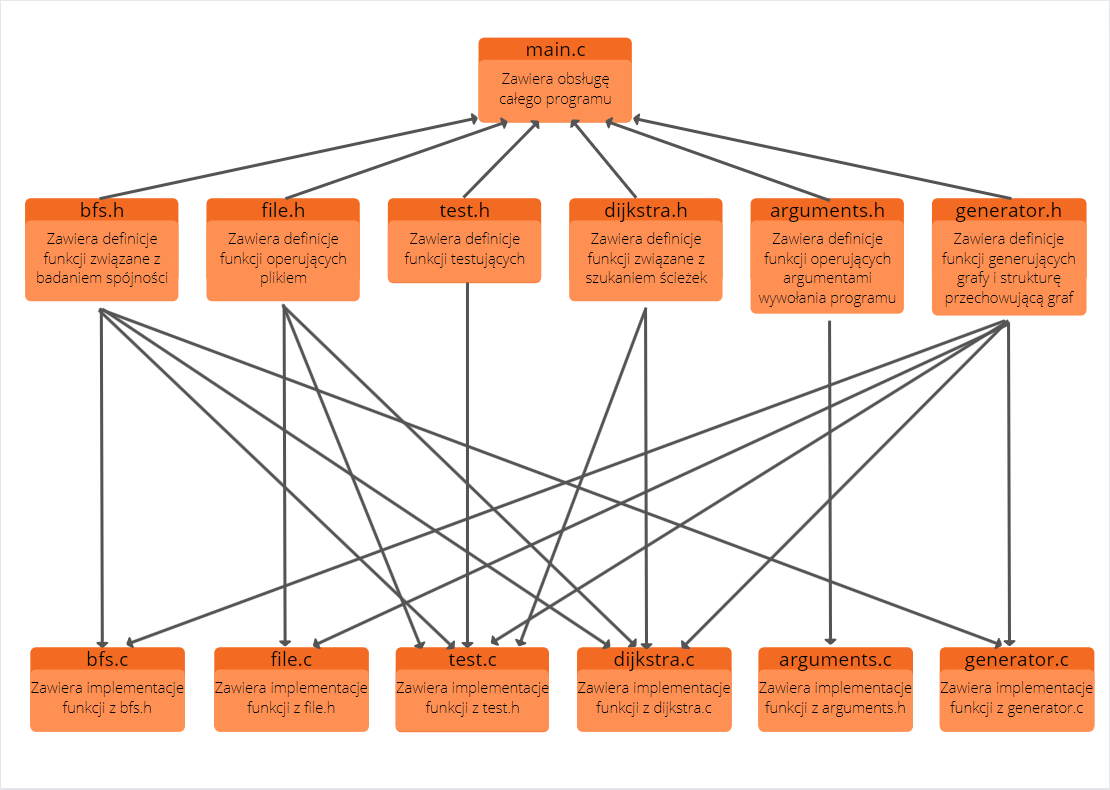
\includegraphics[width=0.9\textwidth]{modularna.png}
\caption{\label{fig:mod}Graficzna reprezentacja struktury programu (opracowanie własne)}
\end{figure}
\begin{itemize}
    

\item main:
    \begin{itemize}
        
    
    \item \texttt{\footnotesize int main(int argc, char** argv)} – odpowiada za całe sterowanie programem
    
    
    \end{itemize}
    
\item generator:
    \begin{itemize}
    \item \texttt{\footnotesize struct tPair} - struktura przechowująca graf
    \item \texttt{\footnotesize void findNeighbours (tPair ** graph, int vertex, int rows, int cols, double minWeight, double maxWeight)} - odpowiada za szukanie sąsiadów poszczególnych wierzchołków
    \item \texttt{\footnotesize void printGraph (tPair ** graph, int n)} - odpowiada za wypisywanie grafu na standardowe wyjście
    tPair ** generateRandWeightMode (int rows, int cols, double minWeight, double maxWeight) - odpowiada za generowanie grafu typu "kartka w kratkę"
    \item \texttt{\footnotesize tPair ** generateAllRandMode (int rows, int cols, double minWeight, double maxWeight)} - odpowiada za generowanie losowego grafu
    \item \texttt{\footnotesize tPair ** generateConMode (int rows, int cols, double minWeight, double maxWeight)} - odpowiada za generowanie spójnego grafu
    \end{itemize}
\item bfs:
    \begin{itemize}
    \item \texttt{\footnotesize struct tQueue} – struktura kolejki dla algorytmu BFS
    \item \texttt{\footnotesize int addToQueue(tQueue* queue, int vertex)} – odpowiada za dodawanie wierzchołka do kolejki
    \item \texttt{\footnotesize int popFromQueue(tQueue* queue)} – odpowiada ze usuwanie wierzchołka z przodu kolejki
    \item \texttt{\footnotesize int BFS(tPair** graph, int n, int startingVertex)} – odpowiada za działanie algorytmu BFS
    \item \texttt{\footnotesize isConst(tPair** graph, int rows, int columns)} – odpowiada za sprawdzenie, czy graf jest spójny
    \end{itemize}
\item arguments:
    \begin{itemize}
    \item \texttt{\footnotesize int readMode (int argc, char **argv)} – odpowiada za ustalenie trybu działania programu
    \item \texttt{\footnotesize int readArgumentsLoadMode (int argc, char **argv, int *pairN, int **pairs, int *generatePairs)} – odpowiada za czytanie argumentów wywołania dla trybu loadMode
    \item \texttt{\footnotesize int readArgumentsRandMode (int argc, char **argv, int *rows, int *cols, double *low, double *high, int *pairN, int **pairs, int *generatePairs, int *doSave, int* doPrintWeights, int *showGraph)} - odpowiada za czytanie argumentów wywołania dla reszty trybów
    \end{itemize}
\item dijkstra:
    \begin{itemize}
    \item \texttt{\footnotesize struct tHeapQueue} – struktura kolejki priorytetowej opartej na kopcu dla algorytmu Dijkstry
    \item \texttt{\footnotesize void heapifyDown(tHeapQueue* heapQueue, double* pathLength)} - odpowiada za naprawienie struktury kopca, po wyjęciu z niego elementu, idąc od korzenia do liści
    int popFromHeapQueue(tHeapQueue* heapQueue, double* pathLength) - wyjęcie najmniejszego elementu z kopca 
    \item \texttt{\footnotesize void heapifyUp(tHeapQueue* heapQueue, double* pathLength)} - odpowiada za naprawienie struktury kopca, po włożeniu do niego elementu, idąc od liści do korzenia
    \item \texttt{\footnotesize void pushToHeapQueue(tHeapQueue* heapQueue, double* pathLength, double vertex)} - włożenie elementu do kopca
    \item \texttt{\footnotesize int isHeapQueueEmpty(tHeapQueue* heapQueue)} - sprawdza czy kolejka priorytetowa jest pusta
    \item \texttt{\footnotesize void printPath(tPair** graph, int* ancestor, int destination, int* path)} – odpowiada za wypisywanie ścieżki
    \item \texttt{\footnotesize void dijkstra (tPair** graph, int pairN, int* pairs, int rows , int cols, int doPrintWeights)} – odpowiada za działanie algorytmu dijkstry
    \end{itemize}

\item file:
    \begin{itemize}
    \item \texttt{\footnotesize tPair ** readFile (char *path, int *rows, int *cols)} - odpowiada za czytanie grafu z pliku
    \item \texttt{\footnotesize void printGraphToFile (tPair ** graph, int rows, int cols)} - odpowiada za zapisywanie grafu do pliku
    \end{itemize}

\item test:
    \begin{itemize}
    \item \texttt{\footnotesize int testRead()} - test czytania grafu
    \item \texttt{\footnotesize int testBFS()} - test działania algorytmu BFS
    \item \texttt{\footnotesize int testDijkstra()} - test działania algorytmu Dijkstry
    \item \texttt{\footnotesize int allTests()} - odpowiada za uruchomienie wszystkich testów
    \item \texttt{\footnotesize int testConModeGenerator()} - test działania generowania grafu w trybie spójności
   \item \texttt{\footnotesize int testAllRandModeGenerator()} - test działania generowania grafu w trybie losowym
    \item \texttt{\footnotesize int testRandWeightModeGenerator()} - test działania generowania grafu w trybie grafu typu "kartka w kratkę"
    
    \end{itemize}


\end{itemize}

\section{Przykładowe wywołania programu}



\subsection {randWeightMode}
Dla prostego wywołania: \texttt{./a.out randWeightMode} otrzymujemy następujący wynik:
 \begin{figure}[htp]
\centering
\includegraphics[width=1\textwidth]{obraz5.png}
\caption{\label{fig:mod}Wynik wywołania w konsoli}
\end{figure}

 
 
W tym wywołaniu nie zostały zdefiniowane żadne parametry poza wybranym trybem działania, dlatego program przyjął standardowe wartości, na podstawie których wygenerował graf typu „kartka w kratkę” oraz 5 par punktów dla których obliczył najkrótszą ścieżkę algorytmem Dijkstry. Program również sprawdził spójność wygenerowanego grafu za pomocą algorytmu BFS. \\ \pagebreak

Jednakże więcej swobody dają wywołania z użyciem zaimplementowanych flag, które pozwalają dowolnie zmieniać parametry programu. \\
Dla przykładowego wywołania z użyciem flag: \texttt{./a.out randWeightMode -r 4 -c 4 -low 10 -high 20 -show -noweights -s -p 2 0 1 4 13} 
\begin{figure}[h]
\centering
\includegraphics[width=1\textwidth]{obraz4.png}
\caption{\label{fig:mod}Wynik wywołania w konsoli}
\end{figure}

Otrzymujemy graf z 4 wierszami i kolumnami, przedziałem wag od 10 do 20 oraz 2 parami (pierwsza liczba po fladze -p) punktów do obliczenia - <0;1> i <4;13>. Dodatkowe flagi -show, -noweights i -s, służą odpowiednio do: wyświetlania wygenerowanego grafu, wypisywania ścieżek bez wag połączeń pomiędzy wierzchołkami oraz do zapisu grafu do pliku o nazwie \texttt{graph-aktualnaData}. \pagebreak

\subsection{allRandMode}
Dla wywołania: \texttt{./a.out allRandMode -r 4 -c 4 -low 10 -high 20 -show -noweights -p 2 0 1 4 13} otrzymujemy: \\
 \begin{figure}[h]
\centering
\includegraphics[width=1\textwidth]{obraz3.png}
\caption{\label{fig:mod}Wynik wywołania w konsoli}
\end{figure}
\\ Zasadniczą różnicą tego trybu jest to, że nie otrzymujemy pełnego grafu „kartka w kratkę” jak poprzednio, lecz tym razem losowane jest, czy dana krawędź w ogóle wystąpi. \pagebreak
\subsection{conMode}
Dla wywołania: \texttt{./a.out conMode -r 4 -c 4 -low 10 -high 20 -show -noweights -p 2 0 1 4 13} otrzymujemy:
\begin{figure}[h]
\centering
\includegraphics[width=1\textwidth]{obraz2.png}
\caption{\label{fig:mod}Wynik wywołania w konsoli}
\end{figure}

 
Tryb conMode oparty jest na trybie allRandMode, z jedyną różnicą, że graf będzie generowany w kółko, aż do momentu, kiedy będzie spójny. \pagebreak
\subsection{loadMode}
Dla wywołania: \texttt{./a.out loadMode isodData 3 0 1 0 2 0 3} otrzymujemy:
 \begin{figure}[h]
\centering
\includegraphics[width=1\textwidth]{obraz1.png}
\caption{\label{fig:mod}Wynik wywołania w konsoli}
\end{figure}

Tryb ten, wczytuje graf z podanego pliku (w tym przypadku „isodData”) i oblicza najkrótsze ścieżki dla podanych par punktów (pierwsza liczba oznacza liczbę par, kolejne liczby to pary punktów).
\pagebreak










\section{Zmiany w ostatecznej wersji względem pierwotnej}

 \begin{figure}[h]
\centering
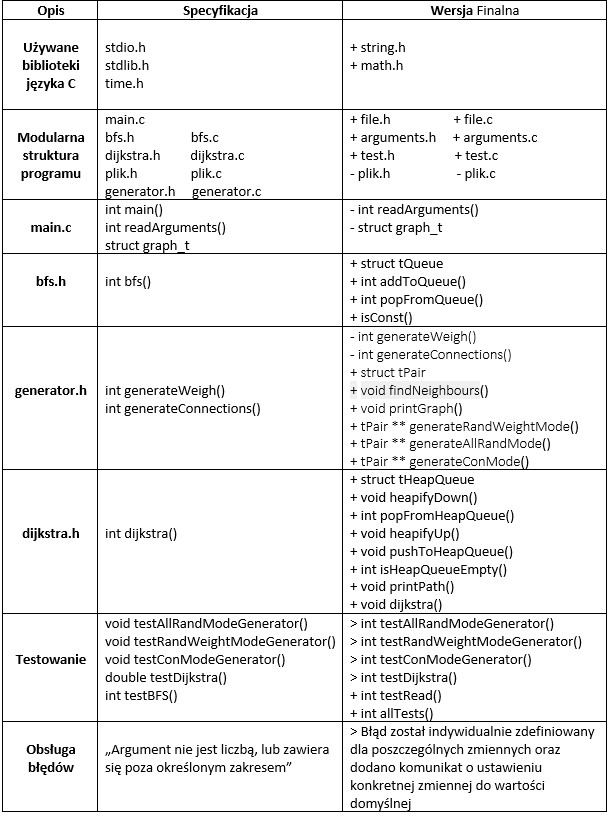
\includegraphics[width=0.8\textwidth]{zmiany.jpg}
\caption{\label{fig:mod}Zmiany wprowadzone w trakcie pracy na projektem w poszczególnych modułach (opracowanie własne)}
\end{figure}




\section{Podsumowanie i wnioski}
 Projekt można uznać za zakończony, a jego finalną wersję ocenić pozytywnie. Nauka, systematyczna praca, wspólna komunikacja oraz wyciąganie odpowiednich wniosków pozwoliły stworzyć program, który całkowicie spełnia założenia jakie sobie postawiliśmy. \\ 
W programie pojawiło się niedużo błędów, przede wszystkim nie testowano poprawności alokowania pamięci przy pomocy funkcji malloc. Cała reszta to kosmetyczne kwestie nie wpływające na samą funkcjonalność, czyli sporadyczna, miejscowa niedokładność lub niespójność formatowania kodu. \\ 
Gdybyśmy mieli pisać ten projekt jeszcze raz, to zdecydowanie stworzylibyśmy strukturę, która przechowuje wszystkie argumenty podawane w linii poleceń, co ułatwiłoby przekazywanie danych do funkcji. Postaralibyśmy się również, aby nie zajmować niepotrzebnie pamięci dla wierzchołków, które nie istnieją, to znaczy powyżej pierwszego wiersza i tym podobnych. Spróbowalibyśmy również napisać cały program w metodyce TDD.  

\section{Przebieg współpracy}
Współpraca przebiegła pomyślnie. Nie pojawiły się żadne problemy z komunikacją. Zasadniczo, nie powstały również żadne konflikty, ponieważ obaj, od samego początku mieliśmy wspólną wizję, według której pracowaliśmy przy projekcie. Implementacja poszczególnych elementów polegała najpierw na rozmowie, a następnie na podziale obowiązków. Regularnie robiliśmy wzajemnie przegląd kodu (code review), a w przypadku problemów z powierzonym zadaniem chętnie sobie pomagaliśmy. \\ 
Pracowaliśmy z pomocą systemu kontroli wersji GIT wykorzystując repozytorium znajdujące się na Projektorze. Każdy z nas miał swoją własna gałąź, na której pracował, a po dokonaniu weryfikacji kodu przez drugą osobę, zmiany były dodawane do gałęzi głównej

\end{document}